\documentclass{standalone}
\usepackage{tikz}
\usetikzlibrary{patterns, positioning}
\usepackage[sfdefault]{ClearSans} %% option 'sfdefault' activates Clear Sans as the default text font
\usepackage[T1]{fontenc}

\begin{document}
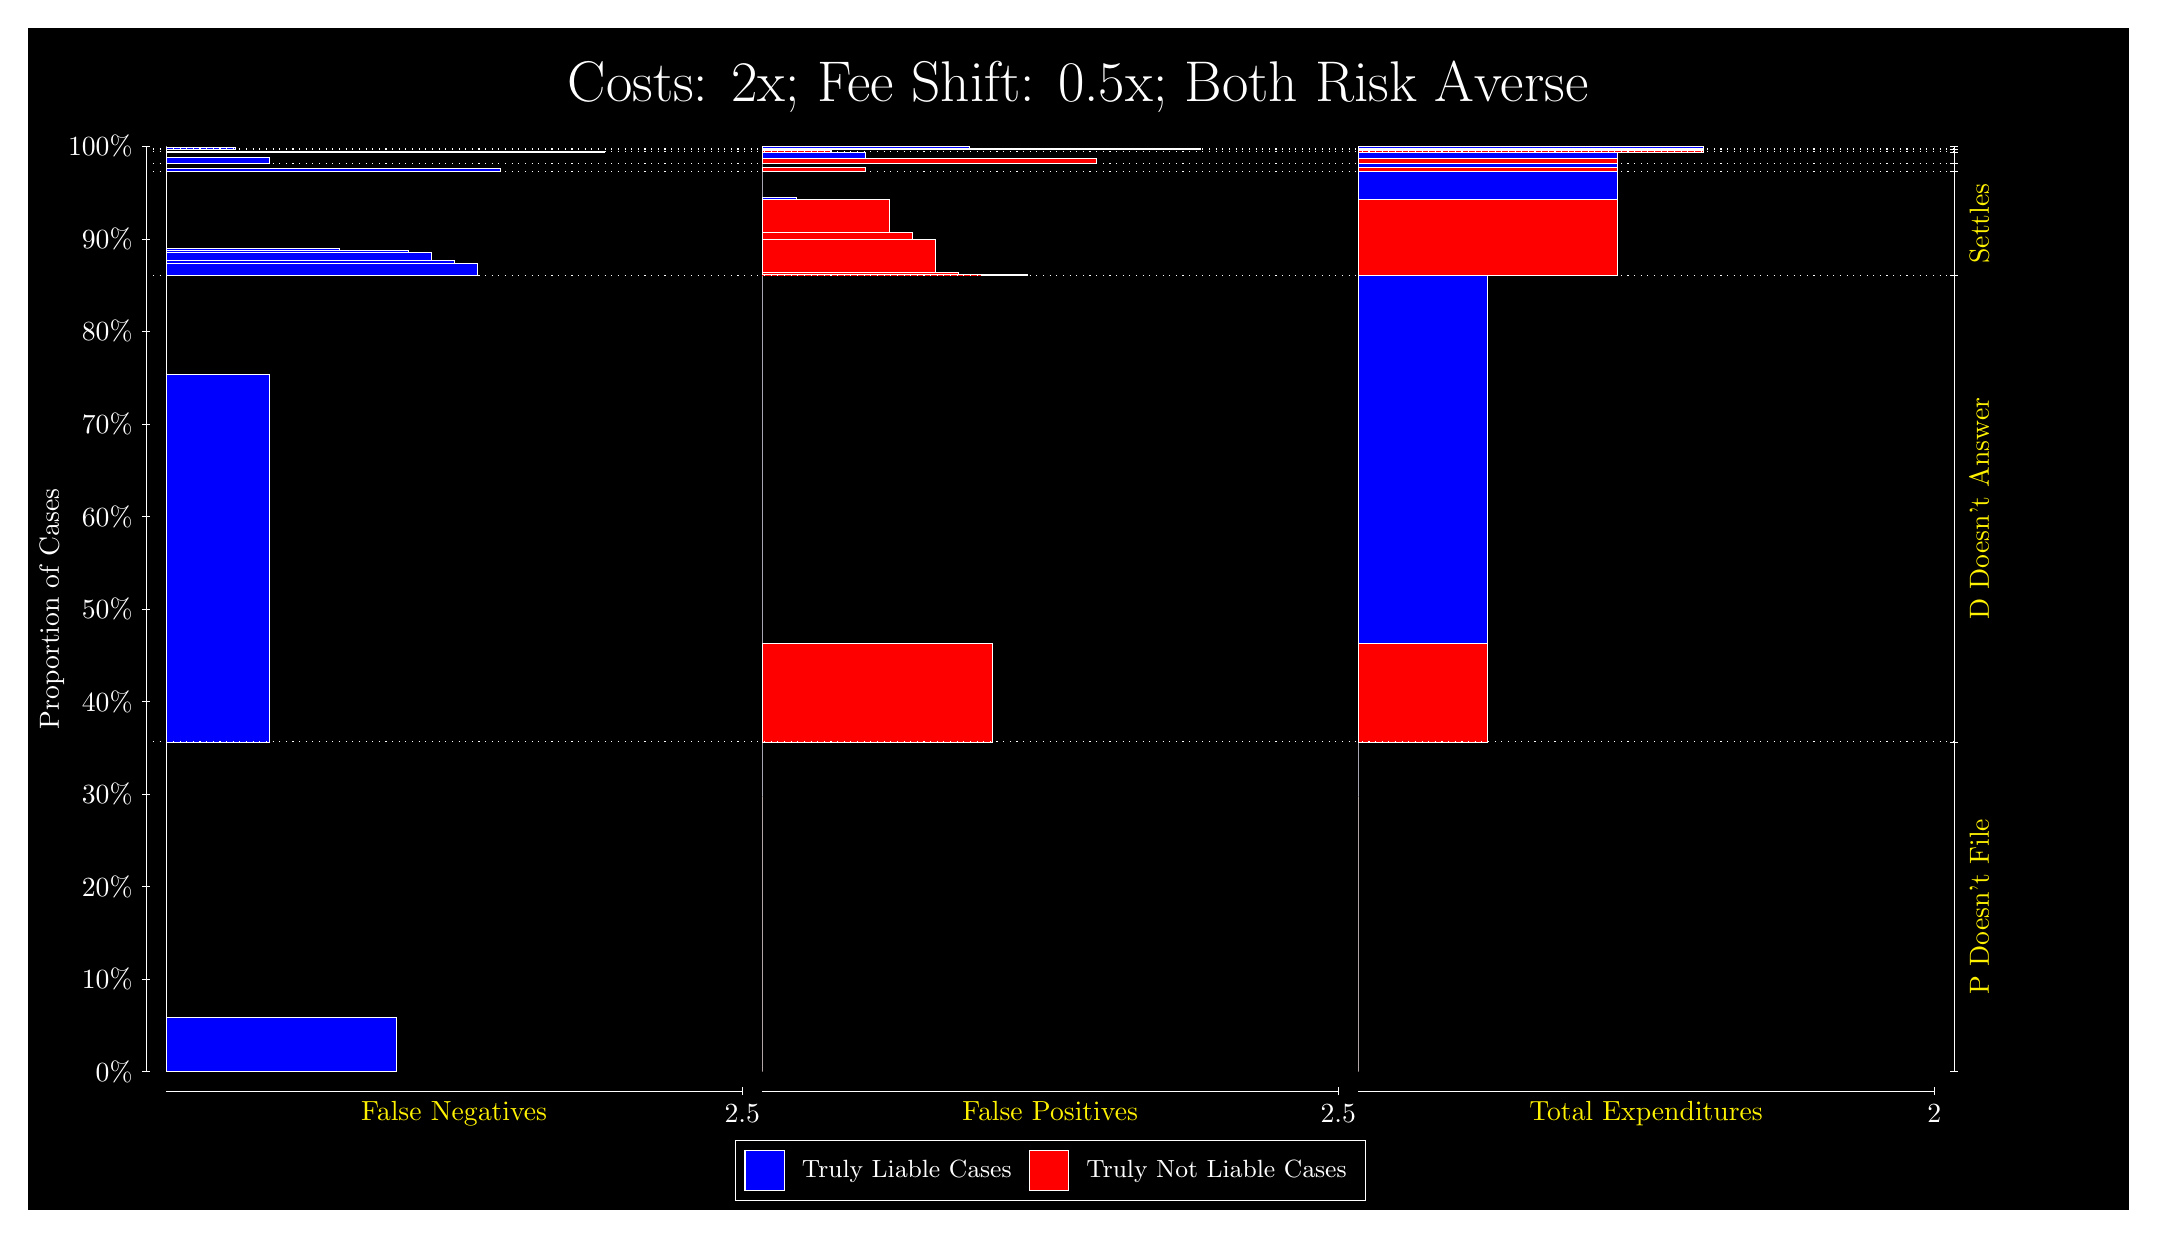
\begin{tikzpicture}
\draw[fill=black] (0,0) rectangle (26.667,15);
\draw[text=white] (0,13.5) rectangle (26.667,15) node[midway] {\huge Costs: 2x; Fee Shift: 0.5x; Both Risk Averse};
\draw[white, very thin] (1.5,1.75) -- (1.5,13.5);
\node[rotate=90, text=white, anchor=center] at (0.3, 7.625) {Proportion of Cases};
\draw[white, very thin] (1.45,1.75) -- (1.55,1.75);
\node[text=white, anchor=east] at (1.45, 1.75) {0\%};
\draw[white, very thin] (1.45,2.925) -- (1.55,2.925);
\node[text=white, anchor=east] at (1.45, 2.925) {10\%};
\draw[white, very thin] (1.45,4.1) -- (1.55,4.1);
\node[text=white, anchor=east] at (1.45, 4.1) {20\%};
\draw[white, very thin] (1.45,5.275) -- (1.55,5.275);
\node[text=white, anchor=east] at (1.45, 5.275) {30\%};
\draw[white, very thin] (1.45,6.45) -- (1.55,6.45);
\node[text=white, anchor=east] at (1.45, 6.45) {40\%};
\draw[white, very thin] (1.45,7.625) -- (1.55,7.625);
\node[text=white, anchor=east] at (1.45, 7.625) {50\%};
\draw[white, very thin] (1.45,8.8) -- (1.55,8.8);
\node[text=white, anchor=east] at (1.45, 8.8) {60\%};
\draw[white, very thin] (1.45,9.975) -- (1.55,9.975);
\node[text=white, anchor=east] at (1.45, 9.975) {70\%};
\draw[white, very thin] (1.45,11.15) -- (1.55,11.15);
\node[text=white, anchor=east] at (1.45, 11.15) {80\%};
\draw[white, very thin] (1.45,12.325) -- (1.55,12.325);
\node[text=white, anchor=east] at (1.45, 12.325) {90\%};
\draw[white, very thin] (1.45,13.5) -- (1.55,13.5);
\node[text=white, anchor=east] at (1.45, 13.5) {100\%};

\draw[white, very thin] (24.457,1.75) -- (24.457,13.5);
\draw[white, very thin] (24.407,1.75) -- (24.507,1.75);
\node[anchor=west] at (24.407, 1.75) {};
\draw[white, very thin] (24.407,5.9367) -- (24.507,5.9367);
\node[anchor=west] at (24.407, 5.9367) {};
\draw[white, very thin] (24.407,11.86) -- (24.507,11.86);
\node[anchor=west] at (24.407, 11.86) {};
\draw[white, very thin] (24.407,13.18) -- (24.507,13.18);
\node[anchor=west] at (24.407, 13.18) {};
\draw[white, very thin] (24.407,13.28) -- (24.507,13.28);
\node[anchor=west] at (24.407, 13.28) {};
\draw[white, very thin] (24.407,13.43) -- (24.507,13.43);
\node[anchor=west] at (24.407, 13.43) {};
\draw[white, very thin] (24.407,13.466) -- (24.507,13.466);
\node[anchor=west] at (24.407, 13.466) {};
\draw[white, very thin] (24.407,13.5) -- (24.507,13.5);
\node[anchor=west] at (24.407, 13.5) {};

\draw[white, very thin, fill=blue] (1.75,1.75) rectangle (4.6775,2.4427);
\draw[white, very thin, fill=red] (1.75,2.4427) rectangle (1.75,5.9367);
\draw[white, very thin, fill=blue] (1.75,5.9367) rectangle (3.0674,10.609);
\draw[white, very thin, fill=red] (1.75,10.609) rectangle (1.75,11.86);
\draw[white, very thin, fill=blue] (1.75,11.86) rectangle (5.7022,12.009);
\draw[white, very thin, fill=blue] (1.75,12.009) rectangle (5.4094,12.053);
\draw[white, very thin, fill=blue] (1.75,12.053) rectangle (5.1167,12.154);
\draw[white, very thin, fill=blue] (1.75,12.154) rectangle (4.8239,12.181);
\draw[white, very thin, fill=blue] (1.75,12.181) rectangle (4.5312,12.182);
\draw[white, very thin, fill=blue] (1.75,12.182) rectangle (3.9457,12.209);
\draw[white, very thin, fill=red] (1.75,12.209) rectangle (1.75,13.18);
\draw[white, very thin, fill=blue] (1.75,13.18) rectangle (5.9949,13.223);
\draw[white, very thin, fill=red] (1.75,13.223) rectangle (1.75,13.28);
\draw[white, very thin, fill=blue] (1.75,13.28) rectangle (3.0674,13.365);
\draw[white, very thin, fill=red] (1.75,13.365) rectangle (1.75,13.43);
\draw[white, very thin, fill=blue] (1.75,13.43) rectangle (7.3123,13.441);
\draw[white, very thin, fill=red] (1.75,13.441) rectangle (1.75,13.466);
\draw[white, very thin, fill=blue] (1.75,13.466) rectangle (2.6283,13.488);
\draw[white, very thin, fill=red] (1.75,13.488) rectangle (1.75,13.5);
\draw[white, very thin, fill=red] (9.3189,1.75) rectangle (9.3189,5.244);
\draw[white, very thin, fill=blue] (9.3189,5.244) rectangle (9.3189,5.9367);
\draw[white, very thin, fill=red] (9.3189,5.9367) rectangle (12.246,7.1881);
\draw[white, very thin, fill=blue] (9.3189,7.1881) rectangle (9.3189,11.86);
\draw[white, very thin, fill=red] (9.3189,11.86) rectangle (12.686,11.87);
\draw[white, very thin, fill=red] (9.3189,11.87) rectangle (12.1,11.871);
\draw[white, very thin, fill=red] (9.3189,11.871) rectangle (11.807,11.898);
\draw[white, very thin, fill=red] (9.3189,11.898) rectangle (11.515,12.317);
\draw[white, very thin, fill=red] (9.3189,12.317) rectangle (11.222,12.414);
\draw[white, very thin, fill=red] (9.3189,12.414) rectangle (10.929,12.831);
\draw[white, very thin, fill=blue] (9.3189,12.831) rectangle (9.758,12.858);
\draw[white, very thin, fill=blue] (9.3189,12.858) rectangle (9.3189,13.18);
\draw[white, very thin, fill=red] (9.3189,13.18) rectangle (10.636,13.238);
\draw[white, very thin, fill=blue] (9.3189,13.238) rectangle (9.3189,13.28);
\draw[white, very thin, fill=red] (9.3189,13.28) rectangle (13.564,13.345);
\draw[white, very thin, fill=blue] (9.3189,13.345) rectangle (10.636,13.43);
\draw[white, very thin, fill=red] (9.3189,13.43) rectangle (10.197,13.454);
\draw[white, very thin, fill=blue] (9.3189,13.454) rectangle (9.3189,13.466);
\draw[white, very thin, fill=red] (9.3189,13.466) rectangle (14.881,13.478);
\draw[white, very thin, fill=blue] (9.3189,13.478) rectangle (11.954,13.5);
\draw[white, very thin, fill=red] (16.888,1.75) rectangle (16.888,5.244);
\draw[white, very thin, fill=blue] (16.888,5.244) rectangle (16.888,5.9367);
\draw[white, very thin, fill=red] (16.888,5.9367) rectangle (18.534,7.1881);
\draw[white, very thin, fill=blue] (16.888,7.1881) rectangle (18.534,11.86);
\draw[white, very thin, fill=red] (16.888,11.86) rectangle (20.181,12.831);
\draw[white, very thin, fill=blue] (16.888,12.831) rectangle (20.181,13.18);
\draw[white, very thin, fill=red] (16.888,13.18) rectangle (20.181,13.238);
\draw[white, very thin, fill=blue] (16.888,13.238) rectangle (20.181,13.28);
\draw[white, very thin, fill=red] (16.888,13.28) rectangle (20.181,13.345);
\draw[white, very thin, fill=blue] (16.888,13.345) rectangle (20.181,13.43);
\draw[white, very thin, fill=red] (16.888,13.43) rectangle (21.279,13.454);
\draw[white, very thin, fill=blue] (16.888,13.454) rectangle (21.279,13.466);
\draw[white, very thin, fill=red] (16.888,13.466) rectangle (21.279,13.478);
\draw[white, very thin, fill=blue] (16.888,13.478) rectangle (21.279,13.5);
\draw[white, dotted] (1.5,5.9367) -- (24.457,5.9367);
\draw[white, dotted] (1.5,11.86) -- (24.457,11.86);
\draw[white, dotted] (1.5,13.18) -- (24.457,13.18);
\draw[white, dotted] (1.5,13.28) -- (24.457,13.28);
\draw[white, dotted] (1.5,13.43) -- (24.457,13.43);
\draw[white, dotted] (1.5,13.466) -- (24.457,13.466);
\draw[white, very thin] (1.75,1.5) -- (9.0689,1.5);
\node[text=yellow, anchor=north] at (5.4094, 1.5) {False Negatives};
\draw[white, very thin] (9.0689,1.45) -- (9.0689,1.55);
\node[text=white, anchor=north] at (9.0689, 1.45) {2.5};

\draw[white, very thin] (9.3189,1.5) -- (16.638,1.5);
\node[text=yellow, anchor=north] at (12.978, 1.5) {False Positives};
\draw[white, very thin] (16.638,1.45) -- (16.638,1.55);
\node[text=white, anchor=north] at (16.638, 1.45) {2.5};

\draw[white, very thin] (16.888,1.5) -- (24.207,1.5);
\node[text=yellow, anchor=north] at (20.547, 1.5) {Total Expenditures};
\draw[white, very thin] (24.207,1.45) -- (24.207,1.55);
\node[text=white, anchor=north] at (24.207, 1.45) {2};

\node[text=yellow, centered, rotate=90] at (24.777, 3.8433) {P Doesn't File};
\node[text=yellow, centered, rotate=90] at (24.777, 8.8985) {D Doesn't Answer};
\node[text=yellow, centered, rotate=90] at (24.777, 12.52) {Settles};





\draw (12.978300999999998,1.5) node[draw=none] (baseCoordinate) {};
\begin{scope}[align=center]
        \matrix[scale=0.5, draw=white, below=0.5cm of baseCoordinate, nodes={draw}, column sep=0.1cm]{
            \node[rectangle, draw, minimum width=0.5cm, minimum height=0.5cm, fill=blue] {}; &
            \node[draw=none, font=\small, text=white] (B) {Truly Liable Cases}; &
            \node[rectangle, draw, minimum width=0.5cm, minimum height=0.5cm, fill=red] {}; &
            \node[draw=none, font=\small, text=white] (B) {Truly Not Liable Cases}; \\
            };
\end{scope}

\end{tikzpicture}
\end{document}